\documentclass[12pt,a4paper]{article}
\usepackage[utf8]{inputenc}
\usepackage[spanish]{babel}
\usepackage{amsmath}
\usepackage{amsfonts}
\usepackage{amssymb}
\usepackage{graphicx}
\usepackage{hyperref}
\usepackage{subfigure}
\usepackage{float}
\usepackage{lscape}
\usepackage{multirow, array} % para las tablas
\usepackage{draftwatermark}
\SetWatermarkText{Lorem ipsum dolor sit amet, consectetur adipiscing elit.}

\begin{document}

\author{Gerardo A. Moreu Vijande}
\title{Colour me Kubrick}
\date{14 de Enero de 2016}
\maketitle

\begin{abstract}
El ejercicio de hoy tratará sobre la inserción de la mayor cantidad posible de comandos en este documento de \LaTeX para ver la destreza del usuario. El contenido mínimo de este documento será de imágenes, listas y tablas, pero todo nuevo comando será bienvenido.  

El tema elegido para este ejercicio es \textbf{Stanley Kubrick\footnote{\url{$https://es.wikipedia.org/wiki/Stanley_Kubrick$}}}, el famoso director británico de cine que jamás ganó un \textit{Óscar} al mejor director pese a haber realizado geniales películas.
\end{abstract}
\tableofcontents
\section{Biografía del autor}
\subsection{Primeros años y vida privada}
Kubrick nació en el barrio neoyorquino del Bronx, en el seno de una familia judía de clase media-alta y a pesar de ello, no tuvo una educación religiosa. Era el primogénito del matrimonio formado por Jacob Leonard Kubrick (1902-1985) y Sadie Gertrude Kubrick, cuyo apellido de soltera fue Perveler. Su hermana Barbara nació en mayo de 1934. Su padre era un doctor con orígenes polacos, austríacos y rumanos, mientras que su bisabuelo Hersh viajó en barco desde Liverpool hasta la Isla de Ellis en 1899, dejando atrás a su esposa e hijos adultos, para iniciar una nueva vida con una mujer mucho más joven que él. Hersh tenía cuarenta y siete años al momento de realizar este viaje.

Stanley mostró desde muy joven su interés por la fotografía, que practicaba con una cámara réflex que le regalaron sus padres. Otra afición eran la música –el jazz en particular; incluso tocó la batería en la Taft Swing Band– y el ajedrez.24 Estos tres pasatiempos serían fundamentales para su futura carrera como director. Su afición a la fotografía le permitió, en primer lugar, trabajar para la revista Look,25 donde hizo reportajes fotográficos a importantes estrellas del momento, y donde se labró una reputación profesional. Su melomanía le permitió a lo largo de toda su carrera poder discutir todos los aspectos relacionados con la banda sonora de sus películas, llegando en ocasiones a prescindir de compositor y escogiendo personalmente piezas de música clásica para sus largometrajes —como en el caso de 2001: A Space Odyssey, descartando en el último momento la banda sonora original de Alex North—. Y su afición al ajedrez quizás pulió el perfeccionismo y la futura frialdad profesional del director. El ajedrez, gracias al cual subsistió durante un inestable período de su vida, sería homenajeado en algunas de sus películas, como The Killing o 2001: A Space Odyssey.

Durante su juventud, Kubrick asistía frecuentemente al cine Loew's Paradise y al Museo de Arte Moderno de Nueva York; también a ver como pasatiempo tardío malas películas que le impulsaron a superarlas con creces. Poco a poco nació la idea de abandonar su trabajo en Look y dedicarse a la realización de películas. Cuando Kubrick aún concedía entrevistas, se refería a Max Ophüls y Sergéi Eisenstein como sus dos referencias cinematográficas más influyentes, el primero por su trabajo con la cámara, y el segundo por su técnica de montaje.

En cuanto a sus relaciones amorosas, Kubrick se casó con su novia de la preparatoria, Toba Metz, el 29 de mayo de 1948, con diecinueve años de edad. Ambos vivieron en Greenwich Village y se divorciaron tres años después. Conoció a su segunda esposa, la bailarina de origen austriaco y diseñadora teatral Ruth Sobotka, en 1952. Vivieron en East Village, se casaron en enero de 1955, se mudaron a Hollywood en julio de ese año y se divorciaron en 1957. Posteriormente, Kubrick se relacionó con la actriz y bailarina Valda Setterfield.

Durante la filmación de Paths of Glory en Múnich, a principios de 1957, Kubrick comenzó una relación con la actriz alemana Christiane Harlan, que tuvo un pequeño papel en dicha película. Ambos se casaron en 1958 y estuvieron juntos por cuarenta años, hasta la muerte del director, en 1999. Además de su hijastra, tuvieron dos hijas juntos; Anya Renata (nacida el 6 de abril de 1959) y Vivian Vanessa (nacida el 5 de agosto 1960).
\subsection{1956-1960: Primera etapa}
\subsection{1960-1968: Consolidación}
\subsection{1968-1980: Obras máximas}
\subsection{1987-1999: Etapa final; la caída y el regreso}
\section{Fallecimiento}
El 7 de marzo de 1999, cuatro días después de una sesión privada para su familia y actores de su último film, Eyes Wide Shut, Kubrick murió de un ataque cardiaco mientras dormía; tenía 70 años. Su funeral se celebró el 12 de marzo en la casa de su finca inglesa, en presencia solo de amigos y familiares cercanos; en total, aproximadamente cien personas. Los medios de comunicación se mantuvieron a una milla de distancia de la puerta de entrada.

Fue enterrado junto a su árbol favorito en Childwickbury Manor, Hertfordshire, Inglaterra. En su libro dedicado a Kubrick, su esposa Christiane incluyó una de las citas favoritas del cineasta, de Oscar Wilde: "La tragedia de la vejez no es que uno sea viejo, sino que sigue siendo joven".
\section{Legado}
Kubrick fue uno de los directores de cine más influyentes en la historia del cine.

Su influencia en el cine contemporáneo es enorme y difícil de definir en su real dimensión. No sólo por la gran cantidad de libros dedicados a su persona y a su trabajo, las compilaciones que lo sitúan entre los más importantes de la historia, así como documentales televisivos sobre su vida y ensayos publicados en diversos medios de comunicación, sino también por los logros fílmicos que alcanzó en vida y el aporte que realizó al statu quo de rol del director dentro la industria cinematográfica.

Kubrick luchó y logró el tan ansiado control total sobre sus películas, con el fin de que su visión fílmica no se viera afectada más que por lo que él entendía como coherencia artística. Sin estudios formales de cine, participó en cada etapa de la producción de una cinta, aprendiendo las técnicas y el oficio, llegando a aportar innovadores procedimientos técnicos (efectos especiales, sistema de filmación, nuevas cámaras, focos, luces y lentes) y narrativos que le permitieron a la industria en general avanzar varios años.

Otro apartado donde fue decisivo fue en el empleo de la banda sonora en las cintas que dirigió, anticipándose a varias tendencias, incorporando tanto la enciclopédica revisión de la música perteneciente a la época en la que se ambientaba la película de turno, así como también emplear los aportes de la electrónica cuando ésta se aplicaba mayormente en el campo experimental.

Sus películas no dejaban de incorporar sus propios intereses intelectuales y la reflexiones sobre el hombre y su lucha constante con su entorno, ya sea físico, social, psicológico o metafísico. Su observación del ser humano siempre guardaba una distancia prudente, que en vez de frialdad (como lo tachaban algunos críticos), podría más bien leerse un verdadero interés y abierta curiosidad por entender el proceder del personaje como pieza dentro de un engranaje más complejo que lo puramente cultural. Él busca aquellos códigos dentro de cada ser humano que lo empujan a accionar de una manera en particular, tanto en la intimidad como en la odiseas titánicas que modifican el curso la historia, creando en el proceso imágenes tan sobresalientes y atemporales que se han convertido en parte de la cultura popular.

Un tema final podría ser su obsesión con los detalles y la calidad del producto. Pocos directores hicieron de esto un tema mayor: entender el filme como acto de aprendizaje extremo del entorno del personaje, sobre la base de una sólida investigación que llevó, junto a su perfeccionismo, a dilatar sus rodajes y aumentar el aura mítica que proyectaba en la prensa.

Además, Kubrick inspiró a directores como Martin Scorsese, Steven Spielberg, James Cameron, Woody Allen, Terry Gilliam, los hermanos Coen, Ridley Scott y George A. Romero. Incluso, Orson Welles comentó: «Entre los que yo llamaría "la generación joven", Kubrick me parece un gigante».

\section{Filmografía }
\begin{enumerate}
\item $\wp$ \textbf{The seafarers}

\item $infty$ \textbf{Fear and desire}

\item $natural$ \textbf{El beso del asesino}

\item $sharp$ \textbf{Atraco perfecto}

\item $Im$ \textbf{Senderos de gloria}

\item $hslash$ \textbf{Espartaco}

\item $\oplus$ \textbf{Lolita}

\item $\blacksquare$ \textbf{Teléfono rojo, ¿volamos hacia Moscú?}

\item $\mho$ \textbf{2001: Una odisea en el espacio \footnote{$http://www.filmaffinity.com/es/film171099.html$}}: La película de ciencia-ficción por excelencia de la historia del cine narra los diversos periodos de la historia de la humanidad, no sólo del pasado, sino también del futuro. Hace millones de años, antes de la aparición del "homo sapiens", unos primates descubren un monolito que los conduce a un estadio de inteligencia superior. Millones de años después, otro monolito, enterrado en una luna, despierta el interés de los científicos. Por último, durante una misión de la NASA, HAL 9000, una máquina dotada de inteligencia artificial, se encarga de controlar todos los sistemas de una nave espacial tripulada.

Trata temas matemáticos mezclándolos con ciertas creencias religiosas budistas, como es la adoración de un \textit{paralelepípedo} negro. Un paralelepípedo (del latín ‘planos paralelos’) es un poliedro de seis caras (por tanto, un hexaedro), en el que todas las caras son paralelogramos, paralelas e iguales dos a dos. Un paralelepípedo tiene 12 aristas, que son iguales y paralelas en grupos de cuatro, y 8 vértices. Su volumen es igual a 
\begin{equation}
\label{v1}
V=\vert a \cdot (b \times c)\vert
\end{equation}
\begin{figure}[htb]
\centering
\subfigure[Paralelepípedo]{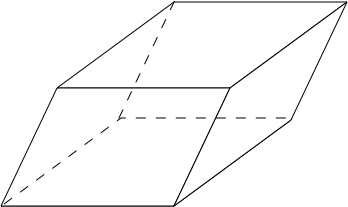
\includegraphics[width=0.45\textwidth]{i1}}
\subfigure[Formas de medir el volumen de la figura]{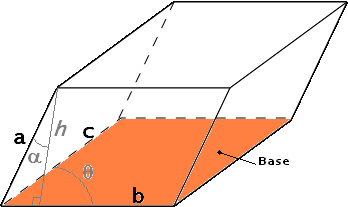
\includegraphics[width=0.45\textwidth]{i2}}
\caption{Paralelepípedo}
\label{paralel}
\end{figure}
La ecuación (\ref{v1}) es equivalente al valor absoluto del determinante de la matriz tridimensional formada por los vectores a, b y c como filas o columnas:
\begin{equation}
\label{v2}
V= \vline \begin{array}{ccc}
a_{x} & a_{y} & a_{z} \\
b_{x} & b_{y} & b_{z} \\
c_{x} & c_{y} & c_{z} \end{array} \vline
\end{equation}

También se habla de la relación entre la evolución de la humanidad y el cuadrado perfecto. Un número cuadrado perfecto en matemáticas, o un número cuadrado, es un número entero que es el cuadrado de algún otro; dicho de otro modo, es un número cuya raíz cuadrada es un número entero.
Un número es un cuadrado perfecto si se puede «ordenar» en una figura cuadrada.

La fórmula más general para el n-ésimo número cuadrado es $n^2$. Este resultado es también igual a la suma de los primeros n números impares, tal y como puede verse en la siguiente fórmula:
\begin{equation}
n^2=\sum_{[k=1]}^n(2 \cdot k -1)
\end{equation}
Por ejemplo, para n=5
\begin{equation}
5^2=\sum_{[k=1]}^5(2 \cdot k -1)= 1 + 3 + 7 + 9 = 25
\end{equation}

\item $\surd$ \textbf{La naranja mecánica}

\item $\clubsuit$ \textbf{Barry Lyndon}

\item $\diamondsuit$ \textbf{El resplandor}

\item $\heartsuit$ \textbf{La chaqueta metálica}

\item $\spadesuit$ \textbf{Eyes Wide Shut}

\end{enumerate}

\subsection{Datos interesantes sobre sus películas}
\begin{landscape} 
\begin{tabular}{|c|c|c|c|c|c|c|}
\hline 
Año & Película & Nominación Óscar & 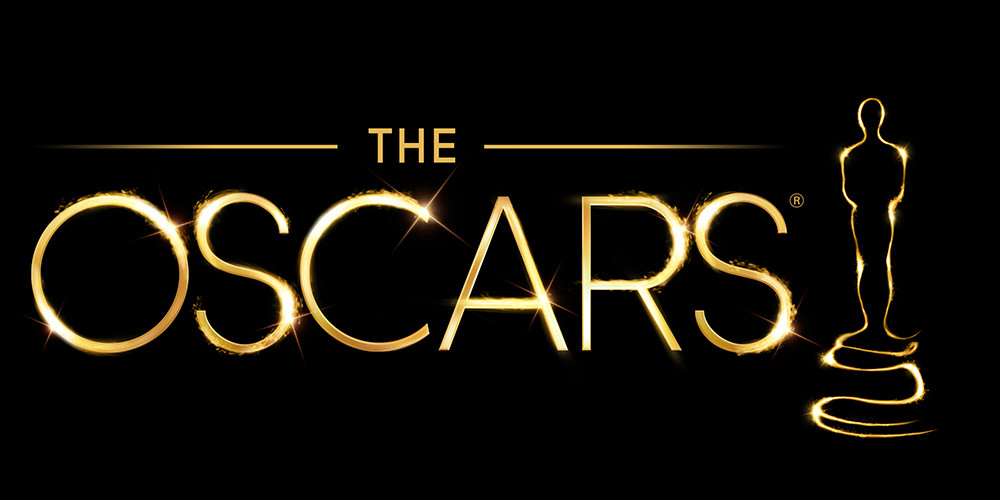
\includegraphics[width=22mm]{Oscar_imagen} & Notas & Presupuesto & IMDB \\ 
\hline 
1951 & Day of the fight & • & x & • & 3900 & • \\ 
\hline 
• & Flying Padre & • & x & • & • & • \\ 
\hline 
1953 & Miedo y deseo & • & x & • & 20000 & 5.7 \\ 
\hline 
• & The seafarers & • & x & • & • & • \\ 
\hline 
1955 & El beso del asesino & • & x & • & 75000 & 6.7 \\ 
\hline 
1956 & Thye killing & • & x & • & • & • \\ 
\hline 
1957 & Senderos de gloria & • & x & • & 935000 & 8.1 \\ 
\hline 
1960 & Espartaco & • & x & • & 12000000 & 7.9 \\ 
\hline 
1962 & Lolita & • & x & • & 2000000 & 7.7 \\ 
\hline 
1964 & Dr. Strangelove & 3 & x & • & 1800000 & 8.5 \\ 
\hline 
1968 & 2001: Una odisea en el espacio & 3 & Efectos visuales & Se rumorea que el escenario  se usó cuando el hombre llegó a la Luna & 10500000 & 8.3 \\ 
\hline 
1971 & La naranja mecánica & 3 & x & • & 2200000 & 8.4 \\ 
\hline 
1975 & Barry Lyndon & 3 & x & • & 11000000 & 8.1 \\ 
\hline 
1980 & El resplandor & • & x & • & 19000000 & 8.4 \\ 
\hline 
1987 & La chaqueta metálica & 1 & x & • & 30000000 & 8.3 \\ 
\hline 
1999 & Eyes Wide Shut & • & x & • & 65000000 & 7.3 \\ 
\hline 
\end{tabular} 
\end{landscape}

\begin{thebibliography}{99}
\bibitem{vida} Esteve Riambau
\emph{Stanley Kubrick. Editorial Catedra, 1990.}

\bibitem{vida2} Michel Ciment
\emph{Kubrick. Ediciones AKAL, 2000.}
\end{thebibliography}

\end{document}
